\documentclass[11pt]{article}
\usepackage{myz310e-notes}
\usepackage{needspace}
\hypersetup{pdftitle={Feed-forward neural networks: from the neuron to the multilayer perceptron},pdfauthor={Emre Onur Kahya},pdfsubject={MYZ 310E Machine Learning in Physics, Fall 2026, lecture note 11 (week 5)}}
\newcommand{\w}{\vect{w}}
\newcommand{\hv}{\vect{h}}
\newcommand{\y}{\vect{y}}
\newcommand{\vt}{\vect{t}}
\newcommand{\va}{\vect{a}}
\newcommand{\vb}{\vect{b}}
\newcommand{\relu}{\operatorname{ReLU}}
\newcommand{\softmax}{\operatorname{softmax}}
\newcommand{\softplus}{\operatorname{softplus}}
\newcommand{\gvec}{\vect{g}}

\begin{document}
\NoteTitle{11}{5}{Feed-forward neural networks:\\ from the neuron to the multilayer perceptron}{Neural networks}{%
Logistic regression is a single artificial neuron, and it draws a hyperplane. Note~10 obtained curved boundaries by
fixing a non-linear feature map in advance; a neural network instead \emph{learns} the feature map, by stacking layers
of neurons and fitting all their weights to the data. This note introduces the artificial neuron and the activation
functions in use today (sigmoid, tanh, ReLU, GELU, SiLU), shows how one hidden layer solves XOR, writes the forward
pass of a multilayer perceptron in matrix form, and matches output units to losses for each task. It then asks what
such networks can represent --- the universal approximation theorem, and why depth can be exponentially more
economical than width --- and which hyperparameters control their capacity. How the gradients are computed
(backpropagation) is the subject of Note~12.}

\section{From biological to artificial neurons}\label{sec:neuron}

A nerve cell receives signals from other cells at thousands of contact points, the \emph{synapses}, on its branched
\emph{dendrites}. Each incoming signal shifts the electrical potential of the cell body by an amount that depends on
the strength of the synapse and may be excitatory or inhibitory. When the summed potential exceeds a threshold, the cell
fires: a voltage pulse, the action potential, travels down its \emph{axon} to the synapses of the next cells. The
human brain holds some $10^{11}$ neurons with of the order of $10^3$ to $10^4$ synapses each, and learning is believed
to work largely by changing synaptic strengths.

The artificial neuron keeps only the arithmetic of this picture: a weighted sum of inputs and a threshold-like
response. Given an input $\x \in \R^d$, weights $\w \in \R^d$ and a bias $b \in \R$, it computes
\begin{equation}\label{eq:neuron}
  a = \w\T\x + b = \sum_{j=1}^d w_jx_j + b, \qquad y = g(a) .
\end{equation}
The number $a$ is the \emph{pre-activation}, and the fixed function $g : \R \to \R$ is the \emph{activation function}
(also called the transfer function or non-linearity). Each weight $w_j$ says how strongly, and with which sign, input
$j$ pushes the output; the bias plays the role of a (negative) threshold. Figure~\ref{fig:neuron} shows the usual
drawing. The biological analogy should not be pushed further: real neurons communicate by spike trains in continuous
time, and the networks of this note are mathematical functions, not brain models.

\begin{figure}[htbp]
\centering
\begin{tikzpicture}[>=Stealth, node distance=1.0cm,
  inp/.style={circle, draw=slate, fill=slate!6, minimum size=7mm, inner sep=0pt},
  unit/.style={circle, draw=indigo, very thick, fill=indigo!6, minimum size=11mm, inner sep=0pt}]
  \node[inp] (x1) at (0, 1.4) {$x_1$};
  \node[inp] (x2) at (0, 0.45) {$x_2$};
  \node at (0, -0.35) {$\vdots$};
  \node[inp] (xd) at (0, -1.2) {$x_d$};
  \node[inp, draw=amber, fill=amber!8] (one) at (1.6, -1.9) {$1$};
  \node[unit] (u) at (3.6, 0.1) {$\Sigma \mid g$};
  \node (y) at (5.6, 0.1) {$y = g(a)$};
  \draw[->] (x1) -- node[above, sloped, font=\small] {$w_1$} (u);
  \draw[->] (x2) -- node[above, sloped, font=\small] {$w_2$} (u);
  \draw[->] (xd) -- node[below, sloped, font=\small] {$w_d$} (u);
  \draw[->, amber] (one) -- node[below right, font=\small] {$b$} (u);
  \draw[->] (u) -- (y);
  \node[font=\small, color=mute, align=left] at (8.6, 0.1) {$a = \w\T\x + b$: pre-activation\\[2pt] $g$: activation function};
\end{tikzpicture}
\caption{An artificial neuron. The bias can be drawn as the weight of a constant input equal to $1$.}
\label{fig:neuron}
\end{figure}

\paragraph{Three neurons we already know} The choice of $g$ turns \eqref{eq:neuron} into familiar models:
\begin{center}\small
\begin{tabular}{@{}L{0.36\linewidth}L{0.16\linewidth}L{0.4\linewidth}@{}}
\toprule
activation $g(a)$ & output & model \\
\midrule
identity, $g(a) = a$ & a real number & linear regression (Note~8) \\
step, $g(a) = \operatorname{sign}(a)$ & $\pm 1$ & perceptron (Note~9, Section~3) \\
sigmoid, $g(a) = \sigma(a) = 1/(1 + e^{-a})$ & a probability & logistic regression (Note~9, Section~4) \\
\bottomrule
\end{tabular}
\end{center}
The neuron is therefore nothing new. What is new in this note is what happens when many of them are combined.

\paragraph{A neuron is a ridge function} The output depends on $\x$ only through the single number $\w\T\x$. Moving
$\x$ in any direction $\vect{u}$ orthogonal to $\w$ leaves $a$, and hence $y$, unchanged: the level sets of a neuron
are the hyperplanes $\w\T\x + b = \text{const}$, and along $\w$ the output follows the profile of $g$. Seen as a
landscape over the input space, a neuron is a ridge or a cliff (Figure~\ref{fig:ridges} of Section~\ref{sec:building}, left).

\begin{worked}{1. One neuron, five activations}
Take $\x = (2, 1, 0.5)$, $\w = (0.5, -1, 2)$ and $b = -0.5$. The pre-activation is
\[
  a = 0.5 \cdot 2 + (-1)\cdot 1 + 2 \cdot 0.5 - 0.5 = 1 - 1 + 1 - 0.5 = 0.5 .
\]
The identity neuron outputs $0.5$; the step neuron outputs $+1$; the sigmoid neuron outputs $\sigma(0.5) = 1/(1 +
e^{-0.5}) = 0.622$; a tanh neuron outputs $\tanh 0.5 = 0.462$; a ReLU neuron (Section~\ref{sec:activations}) outputs
$\max(0, 0.5) = 0.5$. All five give a positive answer, because $a > 0$; they differ in how the answer depends on
$a$. Now move the input along $\vect{u} = (2, 1, 0)$, for which $\w\T\vect{u} = 1 - 1 + 0 = 0$: the point
$\x + s\,\vect{u} = (2 + 2s, 1 + s, 0.5)$ has $a = 0.5$ for every $s$, so every neuron gives the same output all along
this line --- the ridge property.
\end{worked}

\section{Activation functions}\label{sec:activations}

\paragraph{Why a non-linearity at all} Suppose every neuron were linear, $g(a) = a$, and we fed the outputs of a first
layer of neurons, $\hv = W_1\x + \vb_1$, into a second, $\y = W_2\hv + \vb_2$. Then
\[
  \y = W_2(W_1\x + \vb_1) + \vb_2 = (W_2W_1)\,\x + (W_2\vb_1 + \vb_2) ,
\]
again a single linear map: stacking linear layers adds parameters but no expressive power, and any number of layers
collapses to one. Everything interesting in a neural network comes from the non-linear $g$ between the layers.

\paragraph{The classical choices} Table~\ref{tab:act} lists the activation functions met in practice and
Figure~\ref{fig:act} plots them with their derivatives. The \emph{logistic sigmoid} $\sigma$ and the \emph{hyperbolic
tangent} were the standard choices until about 2010. They are smooth, monotone and bounded, and they
\emph{saturate}: for $|a|$ larger than a few units the output is nearly constant and the derivative nearly zero. The
two are the same function up to scaling,
\begin{equation}\label{eq:tanhsig}
  \tanh a = \frac{e^a - e^{-a}}{e^a + e^{-a}} = \frac{1 - e^{-2a}}{1 + e^{-2a}} = \frac{2}{1 + e^{-2a}} - 1 = 2\sigma(2a) - 1 ,
\end{equation}
so a network of tanh units can be rewritten as a network of sigmoid units with rescaled weights (Question~C1). The
differences are practical: tanh is zero-centred, $\tanh 0 = 0$, and its slope at the origin is $1$, four times the
sigmoid's maximal slope $\sigma'(0) = \frac14$. Both derivatives follow from the function value alone,
\[
  \sigma'(a) = \sigma(a)\big(1 - \sigma(a)\big), \qquad
  \tanh'(a) = \frac{(e^a + e^{-a})^2 - (e^a - e^{-a})^2}{(e^a + e^{-a})^2} = 1 - \tanh^2 a ,
\]
the first derived in Note~9, Section~4.1. That a derivative can be computed from the stored output is convenient for
backpropagation (Note~12, Section~3.2).

\begin{table}[htbp]
\centering\small
\caption{Activation functions. $\Phi$ and $\varphi$ are the standard normal distribution function and density.}
\label{tab:act}
\begin{tabular}{@{}lllll@{}}
\toprule
name & $g(a)$ & $g'(a)$ & range & introduced / popularised \\
\midrule
logistic sigmoid & $\sigma(a) = 1/(1 + e^{-a})$ & $\sigma(a)(1 - \sigma(a))$ & $(0, 1)$ & classical \\
hyperbolic tangent & $\tanh a$ & $1 - \tanh^2 a$ & $(-1, 1)$ & classical \\
ReLU & $\max(0, a)$ & $\ind{a > 0}$ & $[0, \infty)$ & \cite{nair2010,glorot2011} \\
leaky ReLU & $\max(\alpha a, a)$, $0 < \alpha < 1$ & $1$ or $\alpha$ & $\R$ & \cite{maas2013} \\
GELU & $a\,\Phi(a)$ & $\Phi(a) + a\,\varphi(a)$ & $[-0.17, \infty)$ & \cite{hendrycks2016} \\
SiLU (swish) & $a\,\sigma(a)$ & $\sigma(a)\big(1 + a(1 - \sigma(a))\big)$ & $[-0.28, \infty)$ & \cite{elfwing2018,ramachandran2017} \\
\bottomrule
\end{tabular}
\end{table}

\begin{figure}[htbp]
\centering
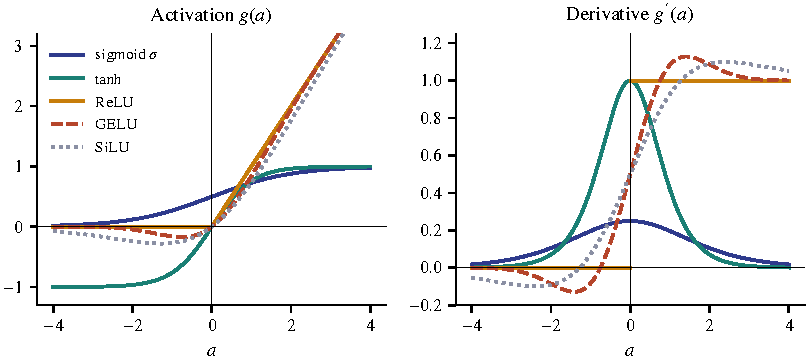
\includegraphics[width=0.94\linewidth]{figures/n11_activations.pdf}
\caption{The activation functions of Table~\ref{tab:act} (left) and their derivatives (right). Sigmoid and tanh
saturate on both sides; ReLU has slope exactly $1$ for $a > 0$ and $0$ for $a < 0$; GELU and SiLU are smooth versions of
ReLU that dip slightly below zero for negative $a$.}
\label{fig:act}
\end{figure}

\paragraph{The rectified linear unit} The ReLU, $\relu(a) = \max(0, a)$~\cite{nair2010,glorot2011}, became the default
for deep networks in the early 2010s. Its derivative is exactly $1$ for every positive input, so it does not saturate
on that side, and it costs a single comparison. For any given input a sizeable fraction of ReLU units output exactly
zero, so the representation is \emph{sparse}. The price is the other side: a unit whose pre-activation is negative for
every training input receives zero gradient and its own weights stop changing; unless the layers below happen to shift
its inputs, it stays silent --- a \emph{dead} unit. The \emph{leaky ReLU} keeps a small slope $\alpha$ (say $0.01$) for
$a < 0$ to avoid this; in the \emph{parametric} ReLU (PReLU)~\cite{he2015} $\alpha$ is itself learned with the weights. The kink at $a = 0$ is harmless: the derivative is
undefined at a single point, which training almost never hits exactly, and libraries simply use $g'(0) = 0$.

\paragraph{Smooth rectifiers} The \emph{Gaussian error linear unit}~\cite{hendrycks2016}, $\mathrm{GELU}(a) =
a\,\Phi(a)$, multiplies the input by the probability that a standard normal variable lies below it: large positive
inputs pass almost unchanged ($\Phi \approx 1$), large negative ones are suppressed ($\Phi \approx 0$), and in between
the gate is soft. The \emph{sigmoid-weighted linear unit} $\mathrm{SiLU}(a) = a\,\sigma(a)$~\cite{elfwing2018}, also
called swish~\cite{ramachandran2017}, does the same with the logistic gate. Both are smooth and slightly
non-monotone, with minima $-0.170$ at $a \approx -0.75$ (GELU) and $-0.278$ at $a \approx -1.28$ (SiLU). Since
$\Phi(a) \approx \sigma(1.702\,a)$, the two curves are close; the tanh-based approximation $\frac12 a\big(1 +
\tanh[\sqrt{2/\pi}\,(a + 0.044715\,a^3)]\big)$ of GELU, used in several implementations, gives $0.84119$ at $a = 1$
against the exact $0.84134$.

\begin{worked}{2. Reading the activations}
At a few pre-activations the functions and their derivatives take the values
\begin{center}\small
\begin{tabular}{@{}rccccccccc@{}}
\toprule
$a$ & $\sigma(a)$ & $\sigma'(a)$ & $\tanh a$ & $\tanh' a$ & $\relu(a)$ & GELU & GELU$'$ & SiLU & SiLU$'$ \\
\midrule
$-2$ & 0.119 & 0.105 & $-0.964$ & 0.071 & 0 & $-0.046$ & $-0.085$ & $-0.238$ & $-0.091$ \\
$-1$ & 0.269 & 0.197 & $-0.762$ & 0.420 & 0 & $-0.159$ & $-0.083$ & $-0.269$ & $0.072$ \\
$0$ & 0.500 & 0.250 & $0$ & 1.000 & 0 & $0$ & $0.500$ & $0$ & $0.500$ \\
$1$ & 0.731 & 0.197 & $0.762$ & 0.420 & 1 & $0.841$ & $1.083$ & $0.731$ & $0.928$ \\
$2$ & 0.881 & 0.105 & $0.964$ & 0.071 & 2 & $1.954$ & $1.085$ & $1.762$ & $1.091$ \\
\bottomrule
\end{tabular}
\end{center}
Three checks. (i) Equation~\eqref{eq:tanhsig} at $a = 1$: $2\sigma(2) - 1 = 2(0.881) - 1 = 0.762 = \tanh 1$.
(ii) $\sigma'(1) = 0.731 \times 0.269 = 0.197$ and $\tanh'(1) = 1 - 0.762^2 = 0.420$: the derivatives follow from the
outputs. (iii) At $a = 2$ the sigmoid passes on only $0.105$ of a small change in its input and tanh only $0.071$,
while ReLU, GELU and SiLU pass on about $1$: in a chain of layers these factors multiply (Note~12, Section~9.2), which is why the
saturating functions make deep networks hard to train. Note also that $\mathrm{SiLU}(a) - \mathrm{SiLU}(-a) =
a\sigma(a) + a\sigma(-a) = a$, the same identity as $\relu(a) - \relu(-a) = a$: both are ``half of the identity'' plus
an even correction.
\end{worked}

\paragraph{Softmax, an output activation} The functions above act on each pre-activation separately. The
\emph{softmax} acts on a whole vector $\va \in \R^m$ and returns a probability vector,
\begin{equation}\label{eq:softmax}
  \softmax(\va)_k = \frac{e^{a_k}}{\sum_{j=1}^m e^{a_j}}, \qquad k = 1, \dots, m ,
\end{equation}
with positive entries summing to one. It is the output layer of every multiclass network. Note~9, Section~4.4 derived
it as multiclass logistic regression, with cross-entropy gradient $\y - \vt$; because adding the same constant to all
scores changes nothing, implementations subtract $\max_j a_j$ before exponentiating. Dividing the scores by a
\emph{temperature} $T > 0$, $y_k \propto e^{a_k/T}$, sharpens ($T < 1$) or flattens ($T > 1$) the distribution (Note~2,
Section~2.2): the scores $\va = (2, 1, 0)$ give $(0.665, 0.245, 0.090)$ at $T = 1$, $(0.867, 0.117, 0.016)$ at
$T = 0.5$ and $(0.367, 0.332, 0.301)$ at $T = 10$. The flattened outputs carry information that a one-hot label does
not: they say which wrong classes the network finds plausible. \emph{Knowledge distillation} exploits this by training
a small ``student'' network to match the softened ($T > 1$) outputs of a large ``teacher''~\cite{hinton2015}.

\begin{physics}{activation functions are thermal averages}
The functions of this section are old friends from statistical mechanics. A spin $s = \pm 1$ in a local field $B$ (measured in energy units), with
energy $-Bs$ at temperature $T$, has Boltzmann probabilities proportional to $e^{\pm\beta B}$ with $\beta =
1/k_BT$, and its mean is
\[
  \langle s \rangle = \frac{e^{\beta B} - e^{-\beta B}}{e^{\beta B} + e^{-\beta B}} = \tanh(\beta B) :
\]
a tanh unit reports the mean orientation of a spin in the field $a$, with $\beta$ absorbed into the weights. The
mean-field equation of the Ising model, $\bar s = \tanh\big(\beta(Jq\bar s + B)\big)$ for the mean spin $\bar s$ and
$q$ neighbours, is a single tanh unit
whose output is fed back as its own input. The occupation of a fermion level of energy $E$, $1/(e^{(E - \mu)/k_BT} +
1) = \sigma\big(-(E - \mu)/k_BT\big)$, is the logistic sigmoid of the Fermi--Dirac distribution, which becomes a step
function as $T \to 0$. The softmax is the Boltzmann distribution over $m$ states with energies $E_k = -a_k$ at $k_BT =
1$; its denominator is the partition function, so $\log\sum_k e^{a_k}$ is minus a free energy, and the softmax
temperature $T$ is literally a temperature. Hopfield's 1982 network~\cite{hopfield1982}, a landmark of the
field, made the link explicit: it is an Ising model whose couplings store memories.
\end{physics}

\begin{modern}{the activations of large language models}
BERT and GPT-2 use GELU in their feed-forward blocks~\cite{devlin2019,radford2019}. Many recent language models use a
\emph{gated} variant, SwiGLU~\cite{shazeer2020}: instead of $W_2\,g(W_1\x)$ the block computes
$W_2\big(\mathrm{SiLU}(W_1\x) \odot (V\x)\big)$, where $\odot$ is the element-wise product and the second matrix $V$
produces a learned, input-dependent gate. LLaMA is an example~\cite{touvron2023}; because the gated block has
three weight matrices instead of two, LLaMA shrinks its hidden width from $4d$ to $\frac23 \cdot 4d$ to keep the number
of parameters unchanged. These choices were made empirically, by comparing validation losses of otherwise identical
models; the theory of this note does not single out a best activation, only the requirement that it be non-linear
(and not a polynomial, Section~\ref{sec:uat}).
\end{modern}

\section{Learning the features}\label{sec:learned}

A sigmoid neuron still draws a hyperplane (Note~9, Section~4.1), as does any monotone $g$ thresholded at a level
it crosses once, and no hyperplane solves XOR (Note~9, Section~6). Of the ``three routes to non-linearity'' of Note~10,
Section~2, the first two compute a map chosen in advance or use it only through its kernel; neural networks take the
third and fit the map itself to the data. Their first layer computes features
\begin{equation}\label{eq:learnedfeat}
  \hv = g(W_1\x + \vb_1) \in \R^{H_1}, \qquad \text{i.e.} \quad h_j = g\big(\w_{1,j}\T\x + b_{1,j}\big),\ \ j = 1, \dots, H_1 ,
\end{equation}
with $g$ applied element-wise, and the second layer is a linear model on $\hv$ --- for classification, logistic or
softmax regression. The difference from Note~10 is that $W_1$ and $\vb_1$ are not fixed in advance: they are fitted to
the data together with the output weights. Each hidden unit $h_j$ is a neuron, so a learned feature is a ridge
function of the input, and the network chooses the directions $\w_{1,j}$ in which the ridges run.

\begin{worked}{3. Two hidden units solve XOR}
Use the $0/1$ form of XOR: $t = 1$ for $(0, 1)$ and $(1, 0)$, $t = 0$ for $(0, 0)$ and $(1, 1)$. Take two ReLU
hidden units that look at the same direction with different thresholds,
\[
  h_1 = \relu(x_1 + x_2), \qquad h_2 = \relu(x_1 + x_2 - 1), \qquad y = h_1 - 2h_2 ,
\]
that is $W_1 = \begin{pmatrix} 1 & 1 \\ 1 & 1 \end{pmatrix}$, $\vb_1 = (0, -1)$, output weights $(1, -2)$ and output bias $0$.
\begin{center}\small
\begin{tabular}{@{}cccccc@{}}
\toprule
$\x$ & $t$ & $x_1 + x_2$ & $(h_1, h_2)$ & $y = h_1 - 2h_2$ & $y > \frac12$\,? \\
\midrule
$(0, 0)$ & 0 & 0 & $(0, 0)$ & 0 & no \\
$(0, 1)$ & 1 & 1 & $(1, 0)$ & 1 & yes \\
$(1, 0)$ & 1 & 1 & $(1, 0)$ & 1 & yes \\
$(1, 1)$ & 0 & 2 & $(2, 1)$ & 0 & no \\
\bottomrule
\end{tabular}
\end{center}
The network reproduces XOR exactly. Figure~\ref{fig:xor} shows why. The hidden layer maps the four inputs to only three
points: $(0, 1)$ and $(1, 0)$ land on the same point $(1, 0)$, and $(1, 1)$ is lifted to $(2, 1)$. In the hidden space
$(h_1, h_2)$ the classes are linearly separable, by the line $h_1 - 2h_2 = \frac12$, and the output unit is an ordinary
linear classifier there. Read back in the input space, the output is the piecewise-linear function of $s = x_1 + x_2$
that rises from $0$ to $1$ on $0 \le s \le 1$ and falls back to $0$ on $1 \le s \le 2$; thresholding it at
$\frac12$ keeps the band $\frac12 < x_1 + x_2 < \frac32$, which contains exactly the two class-1 points. These weights
were set by hand. Gradient training from random initial values often finds an equivalent solution, although with only
two hidden units it can also get stuck (Section~\ref{sec:nonconvex}; Note~12, Section~9).
\end{worked}

\begin{figure}[htbp]
\centering
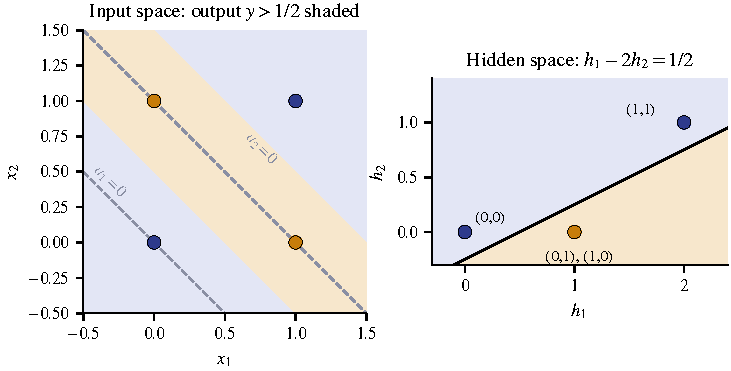
\includegraphics[width=0.8\linewidth]{figures/n11_xor.pdf}
\caption{The XOR network of Worked example~3. Left: input space; the dashed lines are where the hidden pre-activations
vanish, and the shaded band is where the output exceeds $\frac12$. Right: the hidden representation $(h_1, h_2)$, in
which the two inputs of class 1 (amber) coincide and a straight line separates the classes.}
\label{fig:xor}
\end{figure}

\paragraph{Logic gates} With step activations, $g(a) = \ind{a > 0}$, a neuron is a logic gate: $\ind{x_1 + x_2 - 0.5 >
0}$ is OR and $\ind{x_1 + x_2 - 1.5 > 0}$ is AND on binary inputs, and a negative weight implements NOT. XOR is ``OR and
not AND'', so two hidden threshold units and one output unit compute it, which is McCulloch and Pitts's 1943 view of
neurons as logic elements~\cite{mcculloch1943}. Any Boolean function of $d$ inputs is a one-hidden-layer network of
threshold units: give each input pattern of class $1$ its own hidden unit that fires on that pattern only, and let the
output compute their OR. The construction may need up to $2^d$ hidden units, an early warning that ``possible'' and
``economical'' differ (Section~\ref{sec:depth}).

\section{The multilayer perceptron}\label{sec:mlp}

\subsection{One hidden layer}\label{sec:onehidden}

A \emph{multilayer perceptron} (MLP) with one hidden layer of width $H_1$ and $m$ outputs computes
\begin{equation}\label{eq:mlp1}
  \hv = g\big(W_1\x + \vb_1\big), \qquad \y = o\big(W_2\hv + \vb_2\big),
  \qquad W_1 \in \R^{H_1 \times d},\ \vb_1 \in \R^{H_1},\ W_2 \in \R^{m \times H_1},\ \vb_2 \in \R^m ,
\end{equation}
where $g$ is the hidden activation, applied element-wise, and $o$ the output activation (Section~\ref{sec:outputs}).
Written out for one output, $f(\x) = o\big(\sum_{j=1}^{H_1} w_{2,j}\, g(\w_{1,j}\T\x + b_{1,j}) + b_2\big)$: a weighted sum of
$H_1$ ridge functions. The parameters are collected in $\theta = \{W_1, \vb_1, W_2, \vb_2\}$, and their number is
\begin{equation}\label{eq:count1}
  p = H_1(d + 1) + m(H_1 + 1) .
\end{equation}
The inputs form the \emph{input layer}, the $h_j$ the \emph{hidden layer} (hidden because the data never specify their
values), and $\y$ the \emph{output layer} (Figure~\ref{fig:mlp}). Every unit of a layer receives every unit of the layer
below, so these layers are called \emph{fully connected} or \emph{dense}. The network is \emph{feed-forward}: the
connections form no cycle, and information flows from input to output in one pass. The name ``perceptron'' is
historical; the units are not perceptrons with step functions but smooth or piecewise-linear neurons, which is what
makes gradient training possible. Counting conventions differ: this network has one hidden layer but two layers of
weights, and is called a ``two-layer network'' in some books.

\begin{figure}[htbp]
\centering
\begin{tikzpicture}[>=Stealth,
  inp/.style={circle, draw=slate, fill=slate!6, minimum size=7mm, inner sep=0pt},
  hid/.style={circle, draw=indigo, fill=indigo!6, minimum size=7mm, inner sep=0pt},
  outp/.style={circle, draw=amber, fill=amber!8, minimum size=7mm, inner sep=0pt}]
  \foreach \i in {1,2,3} \node[inp] (x\i) at (0, 2.4 - 1.2*\i + 0.6) {$x_\i$};
  \foreach \j in {1,2,3,4} \node[hid] (z\j) at (3.0, 3.0 - 1.2*\j + 0.6) {$h_\j$};
  \foreach \k in {1,2} \node[outp] (y\k) at (6.0, 1.2 - 1.2*\k + 0.6 + 0.6) {$y_\k$};
  \foreach \i in {1,2,3} \foreach \j in {1,2,3,4} \draw[->, draw=mute!70] (x\i) -- (z\j);
  \foreach \j in {1,2,3,4} \foreach \k in {1,2} \draw[->, draw=mute!70] (z\j) -- (y\k);
  \node[font=\small, color=mute, align=center] at (0, -2.75) {input layer\\ $\x \in \R^d$};
  \node[font=\small, color=indigo, align=center] at (3.0, -2.75) {hidden layer\\ $\hv = g(W_1\x + \vb_1)$};
  \node[font=\small, color=amber, align=center] at (6.0, -2.75) {output layer\\ $\y = o(W_2\hv + \vb_2)$};
  \node[font=\small, color=mute] at (1.5, 3.0) {$W_1, \vb_1$};
  \node[font=\small, color=mute] at (4.5, 3.0) {$W_2, \vb_2$};
\end{tikzpicture}
\caption{A multilayer perceptron with $d = 3$ inputs, one hidden layer of $H_1 = 4$ units and $m = 2$ outputs. Each
arrow carries one weight; biases are not drawn. By~\eqref{eq:count1} it has $4 \cdot 4 + 2 \cdot 5 = 26$ parameters.}
\label{fig:mlp}
\end{figure}

Sums of ridge functions can be surprisingly flexible: a handful of hidden units already builds a localised bump, and
sums of bumps approximate any reasonable function (Section~\ref{sec:expressive}).

\paragraph{Matrix form for a mini-batch} Networks are evaluated on many examples at once. Stack the $n'$ inputs of a
mini-batch as the rows of $X \in \R^{n' \times d}$, as in Note~1. The forward pass of \eqref{eq:mlp1} becomes
\begin{equation}\label{eq:batch}
  A_1 = XW_1\T + \vect{1}\vb_1\T, \quad H = g(A_1), \quad A_2 = HW_2\T + \vect{1}\vb_2\T, \quad Y = o(A_2),
\end{equation}
with $H \in \R^{n' \times H_1}$ and $Y \in \R^{n' \times m}$; row $i$ of each matrix belongs to example $i$, and the
products with $\vect{1} \in \R^{n'}$ add the bias to every row (``broadcasting'' in numpy and PyTorch). Each layer is
one matrix product followed by an element-wise function, exactly the operations that GPUs execute fastest.

\begin{worked}{4. A forward pass on a mini-batch of two}
A network with $d = 2$ inputs, $H_1 = 2$ ReLU hidden units and a softmax over $m = 3$ classes has
\[
  W_1 = \begin{pmatrix} 1 & -1 \\ 1 & 1 \end{pmatrix}, \ \ \vb_1 = \begin{pmatrix} 0 \\ -1 \end{pmatrix}, \qquad
  W_2 = \begin{pmatrix} 1 & 0 \\ 0 & 1 \\ -1 & 1 \end{pmatrix}, \ \ \vb_2 = \vect{0} .
\]
The mini-batch holds $\x_1 = (2, 1)$ of class $2$ and $\x_2 = (1, 0)$ of class $1$.

\emph{Hidden layer.} Row by row, $XW_1\T$ contains the dot products of each input with the rows of $W_1$:
\[
  X = \begin{pmatrix} 2 & 1 \\ 1 & 0 \end{pmatrix}, \quad
  A_1 = XW_1\T + \vect{1}\vb_1\T = \begin{pmatrix} 2 - 1 & 2 + 1 \\ 1 - 0 & 1 + 0 \end{pmatrix} + \begin{pmatrix} 0 & -1 \\ 0 & -1 \end{pmatrix}
  = \begin{pmatrix} 1 & 2 \\ 1 & 0 \end{pmatrix} = H .
\]
All pre-activations are non-negative, so the ReLU leaves them unchanged; the second hidden unit sits exactly at its
threshold for $\x_2$ and outputs zero.

\emph{Output layer.} $A_2 = HW_2\T$: for $\x_1$, $(1, 2, -1 + 2) = (1, 2, 1)$; for $\x_2$, $(1, 0, -1 + 0) = (1, 0, -1)$.
The softmax gives
\[
  \y_1 = \frac{(e, e^2, e)}{2e + e^2} = (0.212,\ 0.576,\ 0.212), \qquad \y_2 = (0.665,\ 0.245,\ 0.090) .
\]
The second row equals the softmax of $(2, 1, 0)$ computed in Note~9, Section~4.4, because the scores differ by the constant $1$.

\emph{Loss.} The cross-entropies are $-\log 0.576 = 0.551$ and $-\log 0.665 = 0.408$, and the mini-batch loss is
their mean, $0.480$. Both examples are classified correctly (the largest probability belongs to the true class), but
neither confidently: training would push these probabilities towards $1$.
\end{worked}

\subsection{Deep networks}\label{sec:deep}

Nothing stops us from feeding the hidden layer into another hidden layer. A \emph{deep} MLP with $L$ layers of weights
and widths $H_0 = d, H_1, \dots, H_{L-1}, H_L = m$ computes, starting from $\hv^{(0)} = \x$,
\begin{equation}\label{eq:deep}
  \va^{(k)} = W^{(k)}\hv^{(k - 1)} + \vb^{(k)}, \qquad \hv^{(k)} = g\big(\va^{(k)}\big), \qquad k = 1, \dots, L - 1,
  \qquad \y = o\big(W^{(L)}\hv^{(L - 1)} + \vb^{(L)}\big),
\end{equation}
with $W^{(k)} \in \R^{H_k \times H_{k - 1}}$ and $\vb^{(k)} \in \R^{H_k}$. The function is a composition,
$f = f^{(L)} \circ \dots \circ f^{(1)}$, of simple layer maps, and the number of parameters is
\begin{equation}\label{eq:count}
  p = \sum_{k = 1}^{L} H_k\,(H_{k - 1} + 1) .
\end{equation}
The same letters are used in Notes~12 and~13: layer index $k$, widths $H_k$, pre-activations $\va^{(k)}$, activations
$\hv^{(k)}$, activation function $g$, and $\ell$ for the loss of one example. The intermediate vectors $\hv^{(k)}$ are the network's internal \emph{representations} of the input. In trained
image networks, the early layers respond to local edges and colour contrasts, intermediate layers to textures and
object parts, and late layers to whole objects (Note~13, Section~7, shows how such features are visualised); each layer re-describes the input in terms of the features found by the
layer below. This \emph{hierarchy of representations} is the main idea of deep learning, and it echoes the way physics
describes matter: detector hits are combined into tracks, tracks into particles, particles into the event. The
forward pass is Algorithm~\ref{alg:forward}; it keeps every intermediate $A^{(k)}$ and $H^{(k)}$, because the
backward pass (Note~12, Section~3.4) reuses them.

\begin{algorithm}[htbp]
\caption{Forward pass and prediction of an $L$-layer MLP on a mini-batch}\label{alg:forward}
\begin{algorithmic}[1]
\Require mini-batch $X \in \R^{n' \times d}$; weights $W^{(k)} \in \R^{H_k \times H_{k-1}}$ and biases $\vb^{(k)}$, $k = 1, \dots, L$; hidden activation $g$; output activation $o$
\Function{Forward}{$X$; $\theta$}
  \State $H^{(0)} \gets X$
  \For{$k = 1, \dots, L$}
    \State $A^{(k)} \gets H^{(k - 1)}W^{(k)\mathsf{T}} + \vect{1}\vb^{(k)\mathsf{T}}$ \Comment{matrix product, $O(n'H_{k-1}H_k)$}
    \If{$k < L$} \State $H^{(k)} \gets g(A^{(k)})$ \Comment{element-wise, $O(n'H_k)$}
    \EndIf
  \EndFor
  \State $Y \gets o(A^{(L)})$ \Comment{e.g.\ softmax of each row, $O(n'm)$}
  \State \Return $Y$ and the cache $\{A^{(k)}, H^{(k)}\}$ \Comment{the cache is needed for backpropagation}
\EndFunction
\Function{Predict}{$\x$; $\theta$}
  \State $(Y, \cdot) \gets \textsc{Forward}(\x\T; \theta)$ \Comment{a mini-batch of one; the cache is discarded}
  \State \Return $\argmax_j Y_{1j}$ (classification) or $Y$ itself (regression)
\EndFunction
\end{algorithmic}
\end{algorithm}

\begin{runtime}{forward pass of an MLP}
\emph{Time}: layer $k$ multiplies an $n' \times H_{k - 1}$ matrix by a $H_{k - 1} \times H_k$ matrix,
$n'H_{k - 1}H_k$ multiply--adds; the biases and activations add $O(n'H_k)$. In total
$O\big(n'\sum_k H_{k-1}H_k\big) = O(n'p)$: a few operations per parameter and per example, the assumption made
in Note~7, Section~1. \emph{Prediction}: $O(p)$ per example, independent of the number $n$ of training examples ---
unlike kernel methods (Note~10, Section~9), whose prediction cost grows with $n$. \emph{Memory}: $O(p)$ for the
parameters; during training also $O\big(n'\sum_k H_k\big)$ for the cache of activations, which for wide or deep
networks and large mini-batches often exceeds the memory of the parameters themselves.
\end{runtime}

\begin{worked}{5. Counting parameters and operations}
A classifier for $28 \times 28$ grey-scale digit images has $d = 784$ inputs, hidden layers of widths $512$ and $256$, and
$m = 10$ outputs. By~\eqref{eq:count},
\[
  p = 512\,(784 + 1) + 256\,(512 + 1) + 10\,(256 + 1) = 401\,920 + 131\,328 + 2\,570 = 535\,818 .
\]
All but $512 + 256 + 10 = 778$ of these are weights, so the forward pass of one image costs $535\,040$
multiply--adds, about a million floating-point operations; a mini-batch of $256$ images costs about $2.7 \times 10^8$,
a fraction of a millisecond on a modern GPU. In 32-bit floats the parameters take $535\,818 \times 4$ bytes $\approx 2.1$~MB.
The first layer holds $75\%$ of the parameters: dense layers on raw high-dimensional inputs are expensive, one motivation
for the convolutional layers of Note~13, which share weights across positions.
\end{worked}

\begin{modern}{the MLP inside every transformer}
A transformer layer has two parts: an attention block, which mixes information between the positions of a sequence
(Note~5 related attention to kernel smoothing), and an MLP block, which processes each position separately with the same
one-hidden-layer network, $\hv \mapsto W_2\,g(W_1\hv + \vb_1) + \vb_2$, of hidden width $4d_{\mathrm{model}}$ (or a gated
version, as in the modern box of Section~\ref{sec:activations}). In GPT-2 small~\cite{radford2019}, with
$d_{\mathrm{model}} = 768$ and GELU, each MLP block has $768 \cdot 3072 + 3072 + 3072 \cdot 768 + 768 = 4\,722\,432$
parameters, against $4\,(768^2 + 768) = 2\,362\,368$ for the four projection matrices of attention: two-thirds of the
weights of each of its $12$ layers sit in plain MLPs. Each block is wrapped as $\hv \gets \hv + \mathrm{MLP}(\mathrm{Norm}(\hv))$,
with a \emph{residual connection} and a \emph{normalisation layer}; these two devices, which make very deep stacks
trainable, are introduced in Note~12, Sections~10.2 and~10.3.
\end{modern}

\section{Output units and losses}\label{sec:outputs}

The hidden layers can use any activation; the output layer cannot, because its values must have the meaning that the
task requires: an unbounded number, a probability, a probability vector. The principled way to choose both the output
unit and the loss is maximum likelihood (Note~2, Section~6): let the network output the parameters of a conditional
distribution $p(t \mid \x)$, and minimise the negative log-likelihood $\ell = -\log p(t \mid \x)$ of the observed target.
Table~\ref{tab:outputs} lists the standard pairs; the losses themselves were introduced in Note~4, Section~2.

\begin{table}[htbp]
\centering\small
\caption{Output units and losses. $\va = \va^{(L)}$ is the output pre-activation, $\y = o(\va)$ the output. For every
row the gradient of the loss with respect to $\va$ is $\y - \vt$ (with $\vt$ one-hot for the softmax row).}
\label{tab:outputs}
\begin{tabular}{@{}L{0.16\linewidth}L{0.14\linewidth}L{0.16\linewidth}L{0.2\linewidth}L{0.22\linewidth}@{}}
\toprule
task & target & output unit $o$ & model $p(t \mid \x)$ & loss $\ell$ \\
\midrule
regression & $\vt \in \R^m$ & identity & Gaussian, mean $\y$, fixed variance & $\frac12\norm{\y - \vt}^2$ \\
binary classification & $t \in \{0, 1\}$ & sigmoid & Bernoulli$(y)$ & $-t\log y - (1 - t)\log(1 - y)$ \\
$m$ classes & one-hot $\vt$ & softmax & categorical$(\y)$ & $-\sum_k t_k\log y_k$ \\
multi-label & $\vt \in \{0, 1\}^m$ & $m$ sigmoids & $m$ independent Bernoullis & sum of $m$ binary cross-entropies \\
counts & $t \in \N$ & exponential & Poisson, mean $y$ & $y - t\log y$ \\
\bottomrule
\end{tabular}
\end{table}

\paragraph{Prediction minus target} For each row of Table~\ref{tab:outputs} the derivative of the loss with respect to
the output pre-activation is simply $\y - \vt$. For the identity and squared loss this is immediate, $\partial \ell /
\partial a_k = y_k - t_k$; for the sigmoid with binary cross-entropy and for the softmax it was derived in Note~9,
Sections~4.2 and~4.4. These pairs are not a coincidence. Each target distribution of the table can be written in the
exponential-family form
\[
  p(t \mid a) = \kappa(t)\,e^{at - A(a)}, \qquad A(a) = \log\sum_t \kappa(t)\,e^{at}
\]
(an integral for continuous $t$), with $a$ the output pre-activation: Bernoulli, $\kappa = 1$ and $A(a) = \log(1 + e^a)$;
Poisson, $\kappa(t) = 1/t!$ and $A(a) = e^a$; Gaussian with unit variance, $\kappa(t) = e^{-t^2/2}/\sqrt{2\pi}$ and $A(a) = a^2/2$.
The negative log-likelihood is $\ell = A(a) - at - \log \kappa(t)$, and
\[
  \frac{\partial \ell}{\partial a} = A'(a) - t = \frac{\sum_t t\,\kappa(t)\,e^{at}}{\sum_t \kappa(t)\,e^{at}} - t = \E[t \mid a] - t
  = y - t ,
\]
because the output unit of each row returns exactly the mean: $A'(a) = \sigma(a)$, $e^a$ and $a$ in the three cases
(for the Poisson row, $\ell = e^a - ta + \log t!$ gives $e^a - t$ directly). $A$ is a log partition function, and its
derivative is a mean, exactly as in statistical mechanics (physics box of Section~\ref{sec:activations}); the softmax row
is the same statement with a vector $\va$ and $A(\va) = \log\sum_k e^{a_k}$. Statisticians call such an output unit the
\emph{canonical link} of a generalised linear model. Note~12, Section~2, uses $\y - \vt$ as the starting point of backpropagation.

\paragraph{Squared loss on a sigmoid output} Should a sigmoid output be trained with the squared loss $\ell = \frac12(y -
t)^2$ or with the cross-entropy? With the squared loss the chain rule gives
\begin{equation}\label{eq:sqsig}
  \frac{\partial \ell}{\partial a} = (y - t)\,\sigma'(a) = (y - t)\,y\,(1 - y) ,
\end{equation}
which carries the factor $y(1 - y) \le \frac14$. When the unit saturates on the wrong side --- $y$ close to $0$ while
$t = 1$ --- this factor is tiny, and the gradient vanishes exactly when the error is largest. The cross-entropy cancels
the factor and gives $y - t$, which is large whenever the prediction is badly wrong. The cross-entropy is also the
correct likelihood for a Bernoulli target, while the squared loss corresponds to Gaussian noise on a probability, a
model that makes no sense for $0/1$ labels.

\begin{worked}{6. A saturated output unit}
A sigmoid output unit has $a = -4$ for an example with $t = 1$, so $y = \sigma(-4) = 0.0180$: the network is
confidently wrong. With the squared loss, \eqref{eq:sqsig} gives
\[
  \frac{\partial \ell}{\partial a} = (0.0180 - 1) \times 0.0180 \times 0.9820 = -0.0173 ;
\]
with the cross-entropy, $\partial \ell/\partial a = 0.0180 - 1 = -0.982$, about $57$ times larger. A gradient step on the
squared loss barely moves $a$, and the example is corrected slowly, if at all. At $a = 0$ ($y = \frac12$) the two
gradients are $-0.125$ and $-0.5$: even away from saturation the squared loss is four times weaker.
\end{worked}

\paragraph{Compute losses from the pre-activations} In code, the output activation and the loss are evaluated together
from the \emph{logits} $\va$, never from the probabilities. For a binary output,
\[
  \ell = -t\log\sigma(a) - (1 - t)\log\big(1 - \sigma(a)\big) = t\softplus(-a) + (1 - t)\softplus(a) = \softplus(a) - ta,
\]
with $\softplus(a) = \log(1 + e^a)$, using $-\log\sigma(a) = \log(1 + e^{-a})$, $-\log(1 - \sigma(a)) = \log(1 + e^a)$
and $\softplus(-a) = \softplus(a) - a$. The stable form $\softplus(a) = \max(a, 0) + \log(1 + e^{-|a|})$ never
overflows. The naive route fails already for moderate logits: for $a = 20$ and $t = 0$ the loss is $\softplus(20) =
20.000$, but in 32-bit floats $\sigma(20) = 1 - 2 \times 10^{-9}$ rounds to exactly $1$, and $-\log(1 - y)$ becomes
$-\log 0 = \infty$.
Likewise the multiclass loss is $\log\sum_j e^{a_j} - a_{\mathrm{true}}$, computed after subtracting $\max_j a_j$.
This is why PyTorch's \texttt{CrossEntropyLoss} and \texttt{BCEWithLogitsLoss} take logits as input.

\paragraph{Predicting an error bar} A regression network can output two numbers per target, a mean $\mu(\x)$ and a
log-variance $s(\x) = \log v(\x)$, where $v$ is the predicted variance, and minimise the Gaussian negative log-likelihood
$\frac12\big[(t - \mu)^2e^{-s} + s\big]$ (constant dropped). The first term is the squared error weighted by the
predicted precision, the second stops the network from claiming infinite variance everywhere. Physicists will recognise
the $\chi^2$ of Note~2, Section~3.2, with uncertainties that the network fits and that depend on the input. Such \emph{heteroscedastic} outputs are used, for example, when a
network regresses the energy of a particle shower and must say how precise each estimate is.

\section{What a network can represent}\label{sec:expressive}

\subsection{Building functions from hidden units}\label{sec:building}

In one dimension, a ReLU network with one hidden layer and a linear output computes a continuous function that is
linear between kinks, and every such piecewise-linear function on an interval $[x_0, x_N]$ can be written in this form. Take knots $x_0 < x_1 < \dots < x_N$ and values $f_0,
f_1, \dots, f_N$, write $s_j = (f_{j+1} - f_j)/(x_{j+1} - x_j)$ for the slope on the $j$-th interval, and set
\begin{equation}\label{eq:interp}
  \hat f(x) = f_0 + \sum_{j=0}^{N-1} c_j\,\relu(x - x_j), \qquad c_0 = s_0, \quad c_j = s_j - s_{j-1}\ \ (j \ge 1) .
\end{equation}
On $[x_0, x_1]$ only the first unit is active and $\hat f$ rises from $f_0$ with slope $s_0$; at each knot $x_j$ one more
unit switches on and changes the slope by $c_j$, to $s_j$. So $\hat f$ is the linear interpolant of the points
$(x_j, f_j)$ on $[x_0, x_N]$: $N$ hidden units, one per knot except the last, with input weight $1$, bias $-x_j$ and output weight
equal to the change of slope. The hat function of Figure~\ref{fig:relu}, left, is the special case $\relu(x) -
2\relu(x - 1) + \relu(x - 2)$: slopes $1$, then $-1$, then $0$.

\begin{algorithm}[htbp]
\caption{A one-hidden-layer ReLU network that interpolates given points}\label{alg:interp}
\begin{algorithmic}[1]
\Require knots $x_0 < x_1 < \dots < x_N$ and values $f_0, \dots, f_N$
\Function{ReLUInterpolant}{$\{(x_j, f_j)\}$}
  \For{$j = 0, \dots, N - 1$}
    \State $s_j \gets (f_{j+1} - f_j)/(x_{j+1} - x_j)$ \Comment{slope of piece $j$}
    \State $w_{1,j} \gets 1$; \ $b_{1,j} \gets -x_j$ \Comment{unit $j$ switches on at $x_j$}
    \State $w_{2,j} \gets s_j - s_{j-1}$, with $s_{-1} = 0$ \Comment{change of slope}
  \EndFor
  \State $b_2 \gets f_0$
  \State \Return $(\vect{w}_1, \vb_1, \vect{w}_2, b_2)$ \Comment{$\hat f(x) = \sum_j w_{2,j}\relu(w_{1,j}x + b_{1,j}) + b_2$}
\EndFunction
\end{algorithmic}
\end{algorithm}

\begin{runtime}{constructing the interpolating network}
\emph{Construction}: $O(N)$, one slope and one difference per knot; no optimisation at all. \emph{Prediction}: $O(N)$
per query, one ReLU per hidden unit (a binary search over the knots would find the active piece in $O(\log N)$, but the
network evaluates all units, which on a GPU is the faster option for moderate $N$). \emph{Memory}: $3N + 1$
parameters. The construction is a proof device, not a training method: it needs the values of $f$ at the knots, and in
$d$ dimensions it does not generalise beyond the grid-based bumps discussed below.
\end{runtime}

\begin{worked}{7. Approximating $x^2$ with ReLUs}
Interpolate $f(x) = x^2$ on $[0, 2]$. With the three knots $0, 1, 2$ the values are $0, 1, 4$, the slopes $s_0 = 1$ and
$s_1 = 3$, hence $c_0 = 1$, $c_1 = 2$ and
\[
  \hat f(x) = \relu(x) + 2\,\relu(x - 1) .
\]
Check: $\hat f(1) = 1$, $\hat f(2) = 2 + 2 = 4$. The error is largest at the midpoints of the pieces: $\hat f(0.5) =
0.5$ against $0.25$, $\hat f(1.5) = 1.5 + 1 = 2.5$ against $2.25$, an error of $0.25$. With knot spacing $\Delta = 0.5$
(four units, output weights $0.5, 1, 1, 1$) the maximal error is $0.0625$, and with $\Delta = 0.25$ (eight units) it is
$0.0156$. Halving the spacing doubles the number of units and divides the error by four. In general, linear
interpolation of a twice-differentiable $f$ with spacing $\Delta$ has error at most $\frac18 \Delta^2\max|f''|$ (here
$\frac18 \Delta^2 \cdot 2 = \Delta^2/4$), so $N$ units on a fixed interval give an error of order $1/N^2$. Figure~\ref{fig:relu}, centre, shows
the same for $f(x) = \sin 2x + x/2$ on $[0, \pi]$: maximal error $0.211$ with $4$ pieces and $0.033$ with $12$.
\end{worked}

\begin{figure}[htbp]
\centering
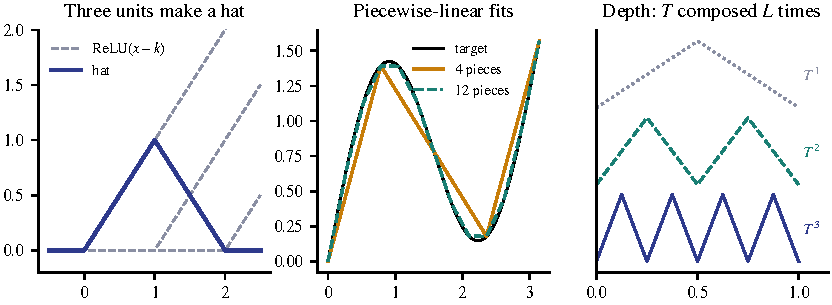
\includegraphics[width=\linewidth]{figures/n11_relu_depth.pdf}
\caption{Left: three ReLU units (dashed) combine into a hat. Centre: one-hidden-layer ReLU networks that interpolate
$\sin 2x + x/2$ at $5$ and $13$ equally spaced knots. Right: the tent map $T(x) = 2\relu(x) - 4\relu(x - \frac12)$ and its
compositions $T^2 = T \circ T$ and $T^3$, offset vertically; $T^L$ has $2^L$ linear pieces (Worked example~8).}
\label{fig:relu}
\end{figure}

\paragraph{Bumps in more dimensions} In one dimension three ReLU units make a hat. In $d$ dimensions every hidden unit
is a ridge that extends without limit along $d - 1$ directions, so a localised bump needs several of them. Figure~\ref{fig:ridges} builds one in two dimensions from sigmoid ridges. A single unit is a smoothed
cliff along its direction $\w$. Two units with the same direction and opposite output weights, $\sigma(4(x_1 + 1)) -
\sigma(4(x_1 - 1))$, give a band, $-1 < x_1 < 1$, running parallel to the $x_2$-axis. Adding the analogous band $-1 <
x_2 < 1$ gives a sum close to $2$ in the central square, close to $1$ on the four arms of a cross, and close to $0$
elsewhere. The output sigmoid matters here: with threshold $1.5$ it is a second non-linearity that cuts away the arms
and keeps only the square. Four hidden units and an output unit thus make a bump, which can be placed anywhere and
made as narrow as desired by scaling the weights. In $d$ dimensions a bump needs $2d$ ridge units, two per coordinate,
and approximating a general function to accuracy $\epsilon$ by bumps on a grid of spacing $\Delta$ needs about
$(1/\Delta)^d$ bumps. For a smooth function and $\epsilon \sim \Delta^2$ that is $\epsilon^{-d/2}$ bumps: the curse
of dimensionality of Note~3, Section~3, in a new form. Constructions of this kind prove what a network \emph{can}
represent; they say nothing about whether that is economical, or whether training finds it.

\begin{figure}[htbp]
\centering
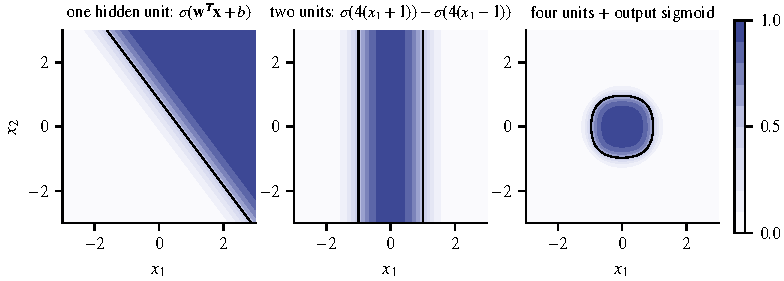
\includegraphics[width=\linewidth]{figures/n11_ridges.pdf}
\caption{Building a bump from ridges. Left: one sigmoid unit, $\sigma\big(4(0.8x_1 + 0.6x_2 - 0.5)\big)$; its level sets
are parallel lines. Centre: the difference of two parallel units is a band. Right: two orthogonal bands (four hidden
units) followed by an output sigmoid, $\sigma\big(8(s - 1.5)\big)$ with $s$ the sum of the two bands, give a localised
bump. Black curves: level $\frac12$.}
\label{fig:ridges}
\end{figure}

\subsection{The universal approximation theorem}\label{sec:uat}

The constructions above extend to a general theorem, proved for sigmoid units by Cybenko~\cite{cybenko1989} and by
Hornik, Stinchcombe and White~\cite{hornik1989}, and later for essentially every activation~\cite{hornik1991,leshno1993}.

\needspace{10\baselineskip}
\begin{keyidea}[Universal approximation]
Let $g : \R \to \R$ be continuous and \emph{not a polynomial}. For every continuous function $f$ on a compact (closed and bounded) set $K
\subset \R^d$ and every $\epsilon > 0$ there exist a width $N$ and parameters $v_j, b_j \in \R$, $\w_j \in \R^d$ such that
\[
  \sup_{\x \in K}\ \Big|\, f(\x) - \sum_{j=1}^N v_j\,g\big(\w_j\T\x + b_j\big) \Big| < \epsilon .
\]
A network with one hidden layer and a linear output can approximate any continuous function on a bounded region
arbitrarily well, provided it has enough hidden units.
\end{keyidea}

\paragraph{Why ``not a polynomial''} If $g$ is a polynomial of degree $r$, then each $g(\w_j\T\x + b_j)$ is a polynomial
of degree at most $r$ in $\x$, and so is any sum of them: the network can never leave this finite-dimensional space,
and cannot approximate, say, $e^{x}$ uniformly on an interval when $r$ is fixed. Any non-polynomial continuous
activation --- sigmoid, tanh, ReLU, GELU, even $\cos$ --- escapes this trap. The theorem extends to vector outputs
(apply it to each component) and to classification: decision regions of any shape can be approximated, which answers
the question raised by XOR.

\paragraph{What the theorem does not say} It is an existence result, and its limitations matter as much as its
statement. (i)~The required width $N$ can be enormous: the bump construction needs a number of units exponential in $d$.
Barron~\cite{barron1993} showed that for functions whose Fourier transform $\hat f(\boldsymbol\omega)$ satisfies $\int\norm{\boldsymbol\omega}\,|\hat
f(\boldsymbol\omega)|\,d\boldsymbol\omega < \infty$ (roughly: $f$ is not dominated by high frequencies) the squared error
of the best width-$N$ network decreases like $1/N$, with a constant that depends on that moment but not explicitly on
$d$ --- a hint that networks can beat grids on suitable function classes. (ii)~It says nothing about
\emph{finding} the weights: training minimises a non-convex objective by gradient descent (Section~\ref{sec:nonconvex};
Note~12, Section~9). (iii)~It says nothing about \emph{generalisation}: with finite data, a network wide enough to approximate
anything can also fit the noise (Note~4, Section~5). Universality is therefore not what distinguishes neural networks:
polynomials, Fourier series and Gaussian-kernel machines (Note~10) are universal too. What matters in practice is how
efficiently a family represents the functions that occur in real problems, and how well gradient training finds them.

\subsection{Depth versus width}\label{sec:depth}

If one hidden layer suffices in principle, why are practical networks deep? Because composition can be exponentially
more economical than addition.

\begin{worked}{8. The tent map: depth beats width}
The tent map on $[0, 1]$ rises linearly from $T(0) = 0$ to $T(\frac12) = 1$ and falls back to $T(1) = 0$. It is a
ReLU network with two hidden units:
\[
  T(x) = 2\relu(x) - 4\relu\big(x - \tfrac12\big) =
  \begin{cases} 2x, & 0 \le x \le \frac12 , \\ 2x - 4(x - \frac12) = 2 - 2x, & \frac12 \le x \le 1 . \end{cases}
\]
Compose it with itself. $T^2 = T \circ T$ sends $[0, \frac14]$ to $[0, 1]$, $[\frac14, \frac12]$ back to $[0, 1]$
(downwards), and so on: two teeth, four linear pieces. For example $T(0.3) = 0.6$, $T^2(0.3) = T(0.6) = 0.8$ and
$T^3(0.3) = T(0.8) = 0.4$. Each composition doubles the number of pieces: every piece is mapped onto $[0, 1]$ and
folded once more. Hence $T^L$ has $2^L$ linear pieces and $2^{L-1}$ teeth
(Figure~\ref{fig:relu}, right), and it is computed by a network of $L$ hidden layers of width $2$: $2L$ hidden units in
all.

A network with \emph{one} hidden layer of $N$ ReLU units computes $\sum_j v_j\relu(w_jx + b_j) + c$, whose slope can
change only at the $N$ points $x = -b_j/w_j$; it has at most $N + 1$ linear pieces. To represent $T^L$ exactly it
therefore needs $N \ge 2^L - 1$ units. For $L = 10$: $20$ hidden units in ten layers, against at least $1\,023$ in one
layer. Telgarsky~\cite{telgarsky2016} turned this example into a theorem: for every $k$ there are functions computed by ReLU
networks with of the order of $k^3$ layers of constant width that no network with at most $k$ layers can even
approximate unless it has of the order of $2^k$ units.
\end{worked}

The number of linear pieces is a crude but telling measure of capacity: for networks with many inputs, the maximal
number of linear regions into which a ReLU network cuts its input space grows exponentially with depth and only
polynomially with width~\cite{montufar2014}. Trained networks use only a fraction of this potential, and the practical
benefit of depth is better described as \emph{reuse}: a feature computed once in a lower layer is shared by every unit
above it, much as the tent map reuses the folding of the previous layer. Functions that occur in nature are often
compositional --- local pieces combined into larger structures --- and deep networks match that structure.

\begin{physics}{networks as variational ansätze and surrogates}
Universal approximation is the reason networks have become a standard \emph{ansatz} in computational physics.
Carleo and Troyer represented the ground-state wave function of a quantum spin system as a small neural network of the
spin configuration and optimised its parameters variationally, reaching accuracies competitive with established
methods on benchmark models~\cite{carleo2017}. Behler and Parrinello wrote the energy of a configuration of atoms as a
sum of atomic energies, each computed by an MLP from rotation- and translation-invariant descriptors of the atom's
neighbourhood~\cite{behler2007}: the same physical idea as the kernel potentials of Note~10, with learned instead of
fixed features. \emph{Physics-informed neural networks}~\cite{raissi2019} go one step further and let an MLP represent
the solution of a differential equation itself (Note~12, Section~10.4). In each case the theorem guarantees that a good
enough network exists; whether a small one exists and can be found is an empirical question for each problem.
\end{physics}

\section{Training and capacity}\label{sec:capacity}

\subsection{The training problem}\label{sec:objective}

Training a network is regularised empirical risk minimisation (Note~4, Section~3.2; Note~7, Section~1):
\begin{equation}\label{eq:objective}
  J(\theta) = \frac1n\sum_{i=1}^n \ell\big(f_\theta(\x_i), \vt_i\big) + \lambda\sum_{k}\norm{W^{(k)}}_F^2 ,
\end{equation}
where $\ell$ is the per-example loss of Table~\ref{tab:outputs}, the penalty sums over all weight matrices,
and $\norm{W}_F^2 = \sum_{jk}W_{jk}^2$. The penalty is called \emph{weight decay}; it usually leaves the biases out
(Note~12, Section~6.1). Note~12 writes it as $\frac{\lambda}{2}\sum_k\norm{W^{(k)}}_F^2$, so its $\lambda$ is twice
ours. There is no closed-form minimiser and $J$ is not convex (Section~\ref{sec:nonconvex}), so it is minimised
iteratively: mini-batch stochastic gradient descent, momentum or Adam (Note~7, Sections~5.3, 6.1 and~6.4), with a
learning-rate schedule such as warm-up followed by cosine decay (Note~7, Section~3.3). The parameters start from small
random values --- not zeros, and not all equal (Note~12, Section~7) --- whose scale matters a great deal. Every step
needs the gradient $\nabla_\theta J$ on a mini-batch. For a network with $p$ parameters, finite differences would cost
$O(p)$ forward passes (Note~7, Section~6.5); \emph{backpropagation} obtains the exact gradient with a backward pass that
costs about twice a forward pass, independently of $p$, and is derived in Note~12, Section~3. The complete loop
(shuffled mini-batches, a gradient step with weight decay, early stopping with patience) is the training loop of
Note~12, Section~5; its stopping rule is the one of Note~7, Section~7.1. For the digit network of Worked example~5 one epoch over
$n = 60\,000$ images costs about $6np \approx 2 \times 10^{11}$ floating-point operations (two per weight and example
forward, about twice that backward), a matter of seconds on a GPU.

\subsection{Hyperparameters that control capacity}\label{sec:hyper}

The weights are fitted on the training set; the choices around them are hyperparameters (Note~4, Section~7). For an
MLP the main ones that set the \emph{capacity} are
\begin{itemize}
\item the \emph{width} $H_k$ of the hidden layers and the \emph{depth} $L$: more units, more functions;
\item the \emph{weight-decay} strength $\lambda$: large weights are needed for sharp transitions (the slope of
  $\sigma(ca)$ at the origin is $c/4$), so penalising them favours smooth functions;
\item the \emph{number of training epochs}: started from small weights, a tanh or sigmoid network is nearly linear
  ($\tanh a \approx a$ for small $a$), and a ReLU network computes a small, gently varying function; the function
  becomes more complex as the weights grow during training, so stopping early limits the capacity actually used
  (Note~7, Section~7.1);
\end{itemize}
and, less directly, the activation function and the optimisation settings (learning rate, mini-batch size, schedule),
which change which of the many minimisers training reaches. They are chosen on a validation set exactly as in
Note~4, Section~7.1 (with $k$-fold cross-validation when data are scarce, Note~4, Section~4.2), using the criterion
that matters, usually the error rate rather than the training cross-entropy. Grid and random search are Note~4,
Section~7.2; advice specific to networks is in Note~12, Section~8.

\begin{figure}[htbp]
\centering
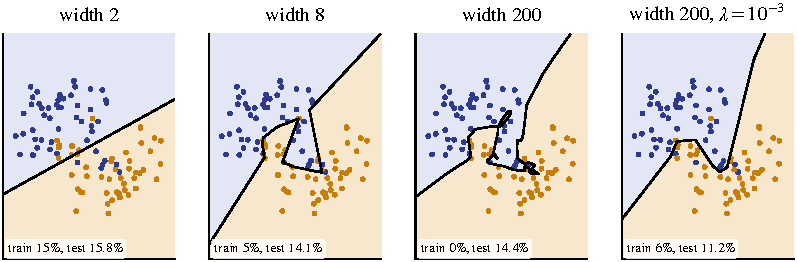
\includegraphics[width=\linewidth]{figures/n11_capacity.pdf}
\caption{One-hidden-layer ReLU networks on $100$ noisy two-moons points, trained by $4000$ full-batch Adam steps
(learning rate $0.01$) on the mean cross-entropy, plus $\lambda\sum_k\norm{W^{(k)}}_F^2$ in the last panel.
Test errors on $5000$ new points.}
\label{fig:capacity}
\end{figure}

Figure~\ref{fig:capacity} varies two of these knobs on the two-moons data of Note~10. With $2$ hidden units the network
can only bend its boundary once (15\% training, 15.8\% test error): it underfits. With $8$ units the boundary follows the
moons (5\%, 14.1\%). With $200$ units and no penalty, training reaches 0\% error by drawing a contorted boundary around
individual points, and the test error rises to 14.4\%: overfitting, the U-shaped curve of Note~4, Section~5. The same
$200$ units with weight decay $\lambda = 10^{-3}$ give a smooth boundary, 6\% training and the best test error, 11.2\%.
A large network with suitable regularisation beat every unregularised width here, which reflects modern practice:
choose a generous architecture and control its capacity by regularisation and early stopping, rather than by making the
network small.


Figure~\ref{fig:epochs} shows the number of epochs at work. The training cross-entropy decreases throughout, to
$0.051$ after $3000$ epochs. The validation cross-entropy reaches its minimum, $0.291$, at epoch $230$ and then grows
to $1.46$, as the network becomes ever more confident on points it has memorised; early stopping on the validation
cross-entropy, as in the training loop of Note~12, Section~5, keeps the parameters of epoch $230$ and gives a test error
of 11.5\%, against 12.8\% at the end. Monitoring the validation error instead would keep the parameters of epoch $340$
(validation error 11.5\%, test error 10.9\%). The validation \emph{error} is flatter and noisier than the validation
cross-entropy: the cross-entropy punishes confident mistakes heavily, whereas the error only counts them. Which
of the two to monitor is itself a choice; the error is what we finally care about, the cross-entropy is less noisy.

\begin{figure}[htbp]
\centering
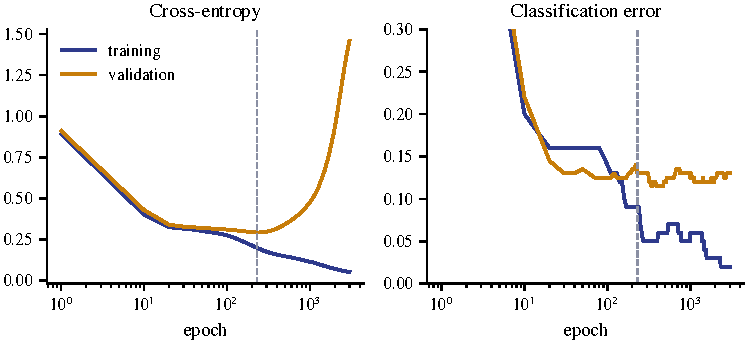
\includegraphics[width=0.86\linewidth]{figures/n11_epochs.pdf}
\caption{Training of the width-$200$ network of Figure~\ref{fig:capacity} without weight decay (full-batch Adam,
learning rate $0.003$), monitored on $200$ validation points. The dashed line marks the epoch of lowest validation
cross-entropy, where early stopping would keep the parameters.}
\label{fig:epochs}
\end{figure}

\begin{modern}{over-parameterised networks}
The width-$200$ network has $801$ parameters for $100$ training points and can fit them perfectly; networks used in
practice are often far more over-parameterised. Zhang and co-authors showed that standard image networks can reach
zero training error even on randomly relabelled data, so their capacity in the classical sense is enormous, yet on real
labels the same networks generalise well~\cite{zhang2017}. The double-descent curve of Note~4, Section~8 is one facet of
this behaviour. In practice large models are trained with AdamW (Note~7, Section~6.4), whose decoupled weight decay is one of
the explicit regularisers, together with early stopping, data augmentation (Note~13, Section~6) and dropout (Note~12, Section~6.3); the
implicit preferences of the optimiser itself contribute as well, and how much each matters is an active research
question.
\end{modern}

\subsection{A non-convex objective}\label{sec:nonconvex}

Logistic regression has a convex loss, so every local minimum is a global one (Note~9, Section~4.3). A network with a
hidden layer does not. Permuting the hidden units of a layer --- swapping rows $j$ and
$k$ of $W_1$ and of $\vb_1$ together with columns $j$ and $k$ of $W_2$ --- changes the parameter vector but not the
function, so every minimiser comes with $H_1!$ copies (more for tanh units, which can flip sign, and a continuous family
for ReLU units, whose weights in and out can be scaled by $c > 0$ and $1/c$). The average of two
such copies gives units $j$ and $k$ identical incoming weights, so they compute the same feature and the network has
effectively lost a unit; in general this midpoint is worse, which a convex $J$ would not allow. Note~12, Section~9
treats the consequences for training.

\begin{physics}{degenerate minima and broken symmetry}
The loss of a network is invariant under the permutation group $S_{H_1}$ of each hidden layer (and, for tanh units,
under the sign flips $\mathbb{Z}_2^{H_1}$), just as the energy of an isotropic ferromagnet is invariant under
rotations of all spins. In both cases the minima are degenerate: a whole orbit of equivalent ground states, of which
the system selects one. Training breaks the symmetry through its random initial condition, as a small stray field
selects the magnetisation direction of a cooling magnet. Why this symmetry must be broken by a random initialisation,
and not left to the training, is shown in Note~12, Section~7.
\end{physics}

\section{Neural networks are back}\label{sec:history}

Neural networks have fallen out of fashion and returned more than once. A short chronology places the ideas of this
note:
\begin{center}\small
\begin{tabular}{@{}lL{0.8\linewidth}@{}}
\toprule
1943 & McCulloch and Pitts describe neurons as threshold logic units~\cite{mcculloch1943}. \\
1958 & Rosenblatt's perceptron learns its weights from examples~\cite{rosenblatt1958} (Note~9, Section~3). \\
1969 & Minsky and Papert analyse what single-layer perceptrons cannot compute, XOR among it~\cite{minsky1969} (Note~9, Section~6); interest declines. \\
1986 & Rumelhart, Hinton and Williams popularise backpropagation for training multilayer networks~\cite{rumelhart1986}
  (reverse-mode differentiation itself is older). \\
1989 & Universal approximation theorems~\cite{cybenko1989,hornik1989}; LeCun and co-workers train a convolutional
  network to read handwritten zip codes~\cite{lecun1989}. \\
1995--2005 & Support vector machines and kernel methods (Note~10), with convex training and few hyperparameters, dominate
  much of machine learning. \\
2006 & Layer-wise pre-training makes deep networks trainable again~\cite{hinton2006}. \\
2010--11 & Rectified linear units~\cite{nair2010,glorot2011}. \\
2012 & AlexNet, a deep convolutional network trained on GPUs, wins the ImageNet challenge by a wide
  margin~\cite{krizhevsky2012} (Note~13, Section~7). \\
2015--16 & Residual networks with over a hundred layers~\cite{he2016} (Note~12, Section~10.3). \\
2017 & The transformer~\cite{vaswani2017}, whose layers alternate attention with the MLP blocks of Section~\ref{sec:deep}. \\
\bottomrule
\end{tabular}
\end{center}
The methods of 2012 differ from those of 1989 less than one might think: an MLP or convolutional network, a
cross-entropy loss, gradients by backpropagation, stochastic gradient descent. What changed was the scale of data (the
ImageNet training set has about $1.2$ million labelled images), the arrival of GPUs, which made the matrix products of
Algorithm~\ref{alg:forward} tens of times faster, and a set of practical improvements: non-saturating activations,
careful initialisation, normalisation layers, residual connections, dropout, and software that computes gradients
automatically (Note~12, Section~3.5). Most of these are the subject of Note~12. The appeal of the kernel methods of the
1990s was a convex problem with a unique answer; the success of networks after 2012 showed that a non-convex problem
whose many minima are all good enough can be the better bargain.

Practical recipes, from input standardisation and the scale of the initial weights to a learning-rate search and a
debugging checklist, are collected in Note~12, Section~10.

\needspace{16\baselineskip}
\begin{keyidea}[Summary]
An artificial neuron computes $g(\w\T\x + b)$; with a sigmoid it is logistic regression and draws a hyperplane. Without
non-linear activations stacked layers collapse to one linear map. Sigmoid and tanh saturate; ReLU, GELU and SiLU do not
for positive inputs and dominate modern practice; the softmax turns scores into probabilities. A multilayer perceptron
computes $\hv^{(k)} = g(W^{(k)}\hv^{(k-1)} + \vb^{(k)})$ layer by layer, a linear model on learned features; it has
$\sum_k H_k(H_{k-1} + 1)$ parameters, and its forward pass costs $O(p)$ per example. Two hidden units solve XOR. The
output unit and the loss are chosen together by maximum likelihood (identity and squared error, sigmoid and binary
cross-entropy, softmax and cross-entropy), and then the gradient with respect to the output pre-activation is $\y - \vt$.
One hidden layer is a universal approximator, but may need exponentially many units; depth can represent some
functions exponentially more compactly. The training objective is regularised empirical risk, non-convex because of the
symmetries of hidden units; width, depth, weight decay and the number of epochs set the capacity and are chosen on
validation data. Gradients come from backpropagation (Note~12).
\end{keyidea}

\begin{questions}
\begin{conceptual}
\item Which three classical models are single artificial neurons, and which activation function gives each? Why is the
  decision boundary of a sigmoid neuron a hyperplane even though $\sigma$ is non-linear?
\item Explain why a network in which every activation is the identity is no more expressive than a single linear layer,
  however many layers and units it has.
\item What does it mean that an activation function saturates? Which functions of Table~\ref{tab:act} saturate, and why
  does saturation slow down gradient-based training?
\item What is a dead ReLU unit? How can it arise during training, and how does the leaky ReLU avoid it?
\item What does dividing the scores of a softmax by a temperature $T > 1$ do to its output? In knowledge distillation,
  why can a student network learn more from the softened outputs of a teacher than from one-hot labels?
\item In Worked example~3, the hidden layer maps $(0, 1)$ and $(1, 0)$ to the same point. Explain why this makes the
  problem linearly separable in the hidden space, and why no hidden layer with a \emph{linear} activation could achieve
  this.
\item For the one-hidden-layer MLP of \eqref{eq:mlp1}, say which parts are chosen by hand and which are fitted to the
  data. Explain why the cost of one of its predictions, unlike that of a kernel method (Note~10), does not grow with
  the number $n$ of training examples.
\item How many parameters does a one-hidden-layer MLP with $d$ inputs, $H_1$ hidden units and $m$ outputs have? Which
  term dominates for image inputs, and what does this suggest about dense layers on raw pixels?
\item Algorithm~\ref{alg:forward} processes a mini-batch with one matrix product per layer instead of a loop over the
  examples. Why does this not change the number of operations, and why is it nevertheless much faster on a GPU?
\item For each of the following tasks, choose the output unit and the loss, and justify the choice by a probabilistic
  model of the target: (a)~predicting the energy of a particle shower; (b)~deciding whether an event is signal or
  background; (c)~identifying which of five particle types produced a track; (d)~tagging an image with any subset of
  20 labels; (e)~predicting the number of photons detected in a time window.
\item Explain why a sigmoid output combined with the squared loss can learn very slowly from examples it gets badly wrong,
  while the cross-entropy does not have this problem.
\item State the universal approximation theorem. Give three things it does \emph{not} guarantee. Why must the activation
  not be a polynomial?
\item Using the tent map, explain why a deep network can represent some functions with far fewer units than a network
  with one hidden layer.
\item Name four hyperparameters that control the capacity of an MLP, and for each explain in which direction it moves
  the network between underfitting and overfitting.
\item In Figure~\ref{fig:epochs}, the validation cross-entropy rises sharply after epoch $230$ while the validation error
  changes little. Explain how this can happen, and discuss which of the two quantities you would use for early
  stopping.
\item Why is the training objective of a network with a hidden layer not convex? Explain the role of the permutation
  symmetry of the hidden units.
\item True or false, with a justification: ``Because one hidden layer is a universal approximator, deep networks are
  never needed.''
\item Give three reasons why neural networks returned to the front of machine learning after 2012, although their basic
  ingredients were known in 1989.
\end{conceptual}

\begin{calculations}
\item A neuron has weights $\w = (1, -2, 0.5)$ and bias $b = 0.5$. For the input $\x = (1, 0.5, 2)$ compute the
  pre-activation and the outputs of a sigmoid, a tanh and a ReLU unit. Verify numerically that $\tanh a = 2\sigma(2a) - 1$
  for your value of $a$. Give a direction $\vect{u} \ne \vect{0}$ along which the output does not change.
\item Using step units $g(a) = \ind{a > 0}$, write down the weights and biases of single neurons computing AND, OR and
  NOT on binary inputs. Combine them into a network with one hidden layer of two units that computes XOR, and check it
  on the four inputs. Then design a network computing XNOR (true when $x_1 = x_2$).
\item An MLP has $d = 100$ inputs, two hidden layers of $64$ units and $10$ outputs. Compute its number of parameters,
  the number of multiply--adds of one forward pass, and the memory needed in 32-bit floats for the parameters alone and
  for parameters, gradient and Adam state together.
\item A three-class softmax output has logits $\va = (1, 3, 0)$ and the true class is the third. Compute the
  probabilities, the cross-entropy and its gradient $\y - \vt$ with respect to the logits, and recompute the
  probabilities at temperature $T = 2$. Then, using the physics box of Section~\ref{sec:activations}: a fermion level lies
  $0.05$~eV above the chemical potential at $k_BT = 0.025$~eV; write its Fermi--Dirac occupation as $\sigma(a)$, and give
  $a$ and the occupation.
\item A sigmoid output unit has pre-activation $a = 3$ for an example with $t = 0$. Compute $\partial \ell/\partial a$ for
  the squared loss $\frac12(y - t)^2$ and for the binary cross-entropy, and their ratio. Repeat for $a = 0$.
\item Write the piecewise-linear interpolant of the points $(0, 0)$, $(1, 2)$, $(2, 1)$, $(3, 3)$ as a one-hidden-layer
  ReLU network (Algorithm~\ref{alg:interp}): give all weights and biases, and check the values at the four knots and at
  $x = 1.5$. Then write $|x|$ (for all real $x$) and $\min(x, 1)$ (for $x \ge 0$) as ReLU networks with two units each.
\item For the tent map $T(x) = 2\relu(x) - 4\relu(x - \frac12)$ compute $T(x)$ and $T^2(x)$ at $x = 0.1$, $0.3$ and
  $0.45$. How many linear pieces does $T^4$ have on $[0, 1]$? How many hidden units does a deep network need to compute
  it, and at least how many a network with one hidden layer?
\needspace{5\baselineskip}
\item A network with $W_1 = \begin{pmatrix} 1 & 0 \\ 1 & -1 \\ 0 & 1 \end{pmatrix}$, $\vb_1 = (0, 0, -1)$, ReLU hidden
  units, output weights $\w_2 = (1, -1, 2)$, output bias $0.5$ and an identity output receives the mini-batch
  $\x_1 = (1, 2)$, $\x_2 = (2, 1)$ with targets $t_1 = 2$, $t_2 = 1$. Compute $A_1$, $H$, the outputs and the mean
  squared loss $\frac{1}{2n'}\sum_i (y_i - t_i)^2$, in the matrix form \eqref{eq:batch}.
\end{calculations}

\begin{derivations}
\item Prove $\tanh a = 2\sigma(2a) - 1$, and derive $\sigma' = \sigma(1 - \sigma)$ and $\tanh' = 1 - \tanh^2$. Show that
  every one-hidden-layer network with tanh hidden units and a linear output computes the same function as a network
  with sigmoid hidden units and a linear output, and give the transformation of the weights and biases.
\item Show that a composition of $L$ affine maps is affine. Then show that a network with identity activations and a
  hidden layer of width $r < \min(d, m)$ represents exactly the affine maps $\x \mapsto M\x + \vect{c}$ with
  $\operatorname{rank} M \le r$.
\item Derive $\partial \ell/\partial a = y - t$ for the sigmoid with binary cross-entropy and for the exponential output
  with the Poisson loss $\ell = y - t\log y$, and derive \eqref{eq:sqsig}. Show that the binary cross-entropy can be written
  as $\softplus(a) - ta$ and that $\softplus(a) = \max(a, 0) + \log(1 + e^{-|a|})$.
\item Prove that the network \eqref{eq:interp} interpolates the points $(x_j, f_j)$, and that a one-hidden-layer ReLU
  network with $N$ units on $\R$ has at most $N + 1$ linear pieces. Using the error bound $\frac18 \Delta^2\max|f''|$ of
  linear interpolation (spacing $\Delta$), find how many units are needed to approximate $\sin x$ on $[0, 2\pi]$ to accuracy $10^{-3}$.
\end{derivations}

\begin{programming}
\item Implement Algorithm~\ref{alg:forward} in numpy for arbitrary widths, ReLU hidden units and a softmax output, using
  only matrix operations. Check it against a loop over examples and units on random inputs, reproduce Worked
  example~4, and measure how the time of a forward pass grows with the width and with the mini-batch size.
\item Using PyTorch (\texttt{torch.nn.Linear}, \texttt{torch.nn.CrossEntropyLoss} or \texttt{BCEWithLogitsLoss} and
  \texttt{torch.optim.AdamW}), train one-hidden-layer networks on noisy two-moons data for widths $2, 8, 32, 200$ and
  several weight-decay values. Reproduce Figures~\ref{fig:capacity} and~\ref{fig:epochs} qualitatively, choose the width,
  the weight decay and the number of epochs on a validation set, and report the test error of your final choice.
\item (a)~Implement Algorithm~\ref{alg:interp} and plot the maximal error of the interpolating network for $f(x) = \sin 2x
  + x/2$ against the number of units on log--log axes; confirm the slope $-2$. (b)~Train one-hidden-layer ReLU networks of
  the same widths by gradient descent on $200$ samples of $f$ and compare their errors with the construction. (c)~Build
  the tent-map network $T^L$ for $L = 1, \dots, 8$ and try to fit $T^6$ with a one-hidden-layer network of $64$ units by
  training. What happens?
\end{programming}
\end{questions}

\paragraph{Further reading} Bishop~\cite{bishop2006}, sections~5.1--5.2; Goodfellow, Bengio and
Courville~\cite{goodfellow2016}, chapter~6; Prince~\cite{prince2023}, chapters~3 and~4, for an excellent visual treatment
of shallow and deep ReLU networks and their linear regions; Murphy~\cite{murphy2022}, chapter~13.

\begin{thebibliography}{99}\small
\bibitem{barron1993} A.~R. Barron, Universal approximation bounds for superpositions of a sigmoidal function, \emph{IEEE Trans.\ Inf.\ Theory} 39, 930--945 (1993).
\bibitem{behler2007} J.~Behler and M.~Parrinello, Generalized neural-network representation of high-dimensional potential-energy surfaces, \emph{Phys.\ Rev.\ Lett.}\ 98, 146401 (2007).
\bibitem{bishop2006} C.~M. Bishop, \emph{Pattern Recognition and Machine Learning}, Springer (2006).
\bibitem{carleo2017} G.~Carleo and M.~Troyer, Solving the quantum many-body problem with artificial neural networks, \emph{Science} 355, 602--606 (2017).
\bibitem{cybenko1989} G.~Cybenko, Approximation by superpositions of a sigmoidal function, \emph{Math.\ Control Signals Systems} 2, 303--314 (1989).
\bibitem{devlin2019} J.~Devlin, M.-W. Chang, K.~Lee and K.~Toutanova, BERT: pre-training of deep bidirectional transformers for language understanding, \emph{NAACL} (2019).
\bibitem{elfwing2018} S.~Elfwing, E.~Uchibe and K.~Doya, Sigmoid-weighted linear units for neural network function approximation in reinforcement learning, \emph{Neural Netw.}\ 107, 3--11 (2018).
\bibitem{glorot2011} X.~Glorot, A.~Bordes and Y.~Bengio, Deep sparse rectifier neural networks, \emph{AISTATS} (2011).
\bibitem{goodfellow2016} I.~Goodfellow, Y.~Bengio and A.~Courville, \emph{Deep Learning}, MIT Press (2016).
\bibitem{he2015} K.~He, X.~Zhang, S.~Ren and J.~Sun, Delving deep into rectifiers: surpassing human-level performance on ImageNet classification, \emph{ICCV} (2015).
\bibitem{he2016} K.~He, X.~Zhang, S.~Ren and J.~Sun, Deep residual learning for image recognition, \emph{CVPR} (2016).
\bibitem{hendrycks2016} D.~Hendrycks and K.~Gimpel, Gaussian error linear units (GELUs), arXiv:1606.08415 (2016).
\bibitem{hinton2006} G.~E. Hinton, S.~Osindero and Y.-W. Teh, A fast learning algorithm for deep belief nets, \emph{Neural Comput.}\ 18, 1527--1554 (2006).
\bibitem{hinton2015} G.~Hinton, O.~Vinyals and J.~Dean, Distilling the knowledge in a neural network, arXiv:1503.02531 (2015).
\bibitem{hopfield1982} J.~J. Hopfield, Neural networks and physical systems with emergent collective computational abilities, \emph{Proc.\ Natl.\ Acad.\ Sci.\ USA} 79, 2554--2558 (1982).
\bibitem{hornik1989} K.~Hornik, M.~Stinchcombe and H.~White, Multilayer feedforward networks are universal approximators, \emph{Neural Netw.}\ 2, 359--366 (1989).
\bibitem{hornik1991} K.~Hornik, Approximation capabilities of multilayer feedforward networks, \emph{Neural Netw.}\ 4, 251--257 (1991).
\bibitem{krizhevsky2012} A.~Krizhevsky, I.~Sutskever and G.~E. Hinton, ImageNet classification with deep convolutional neural networks, \emph{NeurIPS} (2012).
\bibitem{lecun1989} Y.~LeCun, B.~Boser, J.~S. Denker, D.~Henderson, R.~E. Howard, W.~Hubbard and L.~D. Jackel, Backpropagation applied to handwritten zip code recognition, \emph{Neural Comput.}\ 1, 541--551 (1989).
\bibitem{leshno1993} M.~Leshno, V.~Ya.~Lin, A.~Pinkus and S.~Schocken, Multilayer feedforward networks with a nonpolynomial activation function can approximate any function, \emph{Neural Netw.}\ 6, 861--867 (1993).
\bibitem{maas2013} A.~L. Maas, A.~Y. Hannun and A.~Y. Ng, Rectifier nonlinearities improve neural network acoustic models, \emph{ICML Workshop on Deep Learning for Audio, Speech and Language Processing} (2013).
\bibitem{mcculloch1943} W.~S. McCulloch and W.~Pitts, A logical calculus of the ideas immanent in nervous activity, \emph{Bull.\ Math.\ Biophys.}\ 5, 115--133 (1943).
\bibitem{minsky1969} M.~Minsky and S.~Papert, \emph{Perceptrons}, MIT Press (1969).
\bibitem{montufar2014} G.~Mont\'ufar, R.~Pascanu, K.~Cho and Y.~Bengio, On the number of linear regions of deep neural networks, \emph{NeurIPS} (2014).
\bibitem{murphy2022} K.~P. Murphy, \emph{Probabilistic Machine Learning: An Introduction}, MIT Press (2022).
\bibitem{nair2010} V.~Nair and G.~E. Hinton, Rectified linear units improve restricted Boltzmann machines, \emph{ICML} (2010).
\bibitem{prince2023} S.~J.~D. Prince, \emph{Understanding Deep Learning}, MIT Press (2023).
\bibitem{radford2019} A.~Radford, J.~Wu, R.~Child, D.~Luan, D.~Amodei and I.~Sutskever, Language models are unsupervised multitask learners, OpenAI technical report (2019).
\bibitem{raissi2019} M.~Raissi, P.~Perdikaris and G.~E. Karniadakis, Physics-informed neural networks: a deep learning framework for solving forward and inverse problems involving nonlinear partial differential equations, \emph{J.\ Comput.\ Phys.}\ 378, 686--707 (2019).
\bibitem{ramachandran2017} P.~Ramachandran, B.~Zoph and Q.~V. Le, Searching for activation functions, arXiv:1710.05941 (2017).
\bibitem{rosenblatt1958} F.~Rosenblatt, The perceptron: a probabilistic model for information storage and organization in the brain, \emph{Psychol.\ Rev.}\ 65, 386--408 (1958).
\bibitem{rumelhart1986} D.~E. Rumelhart, G.~E. Hinton and R.~J. Williams, Learning representations by back-propagating errors, \emph{Nature} 323, 533--536 (1986).
\bibitem{shazeer2020} N.~Shazeer, GLU variants improve transformer, arXiv:2002.05202 (2020).
\bibitem{telgarsky2016} M.~Telgarsky, Benefits of depth in neural networks, \emph{COLT} (2016).
\bibitem{touvron2023} H.~Touvron \emph{et al.}, LLaMA: open and efficient foundation language models, arXiv:2302.13971 (2023).
\bibitem{vaswani2017} A.~Vaswani \emph{et al.}, Attention is all you need, \emph{NeurIPS} (2017).
\bibitem{zhang2017} C.~Zhang, S.~Bengio, M.~Hardt, B.~Recht and O.~Vinyals, Understanding deep learning requires rethinking generalization, \emph{ICLR} (2017).
\end{thebibliography}

\SourceNote
\end{document}
